\section{HR Simulation}
\label{sec:HRsim}
The HR simulation handles all parts of the Human Resources Process which are described in the following subchapters.
\subsection{Employee types}
The following list shows possible employee types that can be hired. The role of HR, Finance and Marketing is performed by the player itself, thus not requiring employees in these departments.
\begin{itemize}
    \item Engineers % instead of Production
    %\item Logistics --> not needed, included in Trucks
    \item Salespeople \\
    fsdfdsafsfa
    %\item Support --> only external partners
    %\item Marketing --> not needed
\end{itemize}

\subsection{Hiring / Firing}
The HR process starts with hiring human resources. Therefore, available engineers and salespeople need to be chosen from the market. Each employee has a requested salary. Moreover, hiring and also firing of employees is associated with cost of 5000 \$. \cite{recruiterbox}

\subsection{Key Performance Indicators}
\label{sub:KPI}
\subsubsection{Job Satisfaction}
The job satisfaction is an essential part of a Key Performance Indicator framework in order to measure the management quality of the player. Many different parts in the cooperation depend on the job satisfaction of employees, thus, in order to increase the performance, managers need to make sure that the satisfaction of their employees is constantly high.\cite{KOYS}

The job satisfaction is such an important factor due to the fact that the employer branding is influenced by it. This is critical as the employer branding has a huge impact on how the company is perceived on the markets by potential employees but also by customers and suppliers. Moreover, the employer branding is also influenced by the general company image and can be influenced through marketing and PR activities. 

The success of a company highly depends on the ability of attracting the best people. The ease of recruitment is highly dependent on the job satisfaction of the employees. Extrinsic motivation needs to be provided to attract employees in case the job satisfaction and by this the employer branding are low. A low job satisfaction makes it necessary to pay higher salaries. Not only the recruiting of employees is more difficult with a lower job satisfaction but also the employee turnover is higher. \cite{frederiksen2016}

Different factors exist which influence the job satisfaction. \cite{Kapur} The implementation and integration of softfactors which influence the job satisfaction was not the primary goal for CapX, we concentrated on the hardfactors which include Salary and Paymix, Worktime, the Skills and Education and the provided Benefits by the company. 

The following table shows the possible influencing factors which can be chosen by the player to influence the employees job satisfaction. The monetary impact is counted in dollars per employee per month. 

\begin{table}[]
    \centering
\begin{tabular}{l|c|c}
    \hline
     \textbf{Benefit} & \textbf{Points} & \textbf{Monetary impact} \\
     \hline \hline
     \multicolumn{1}{c|}{\underline{\textbf{Salary}}} & & \\
     Salary below average & 0 &  \\
     Salary on average & 2 &  \\
     Salary above average & 4 &   \\
     \hline
     \multicolumn{1}{c|}{\underline{\textbf{Worktime}}} & & \\
     6 hours & 4 & -100\$  \\
     8 hours & 2 & 0\$  \\
     10 hours & 0 & 80\$  \\
     \hline
     \multicolumn{1}{c|}{\underline{\textbf{Company Car}}} & & \\
     Not offered & 0 & -100\$  \\
     Medium Size & 2 & 0\$  \\
     Full Size & 4 & 80\$  \\
     \hline
     \multicolumn{1}{c|}{\underline{\textbf{Home Office (HO)}}} & & \\
     Fixed Model & 0 & 0\$  \\
     Flextime model & 1 & 100\$  \\
     Trust-based (TB) & 2 & 200\$  \\
     Trust-based (TB) + HO one time per week & 3 & 280\$  \\
     Trust-based (TB) + always HO allowed & 4 & 350\$  \\
     \hline
     \multicolumn{1}{c|}{\underline{\textbf{IT Equipment}}} & & \\
     High End & 4 & -50\$  \\
     Market Average & 0 & 0\$  \\
     \hline
     \multicolumn{1}{c|}{\underline{\textbf{Food / Coffee}}} & & \\
     Offered for free & 4 & -100\$  \\
     Employee payment & 0 & 0\$  \\
     \hline
     \multicolumn{1}{c|}{\underline{\textbf{Gym / Sports}}} & & \\
     Offered for free & 4 & -100\$  \\
     Not offered & 0 & 0\$  \\
     \hline

\end{tabular}
\caption{Benefits influencing the Job Satisfaction}
    \label{tab:benefitsJSS}
\end{table}

For each of the above mentioned categories (Salary, Worktime, Company Car, Homeoffice, IT Equipment, Food and Sports) the player needs to make a decision which benefit category to offer. The numbers in brackets show the points which adds up to a total job satisfaction score after the player made all necessary choices. The job satisfaction score can have a minimum of 0 points and a maximum of 28 points.

As this scale is too simple in order to be somehow realistic, a manipulation of the original scale is needed. The marginal impact of an additional increase of factors which lead to a higher job satisfaction decreases over time, e.g. an employee which has an above average salary, a company car, trusted based working hours and all other benefits on the highest level, would not value the additional offering of a free sports club voucher as much as an employee that has no benefits at all and gets a sports club voucher. Thus the scale of 0 - 28 was transformed to a root function.

Moreover, the job satisfaction also depends on the level of the employee. Each employee has its own specific requirements and expectations. Generally, we assume that employees with a lower skill level who are younger, are more easily satisfied than employees with a higher skilllevel. In this case the skilllevel  is used as a proxy for the expectations of an employee towards the employer. 

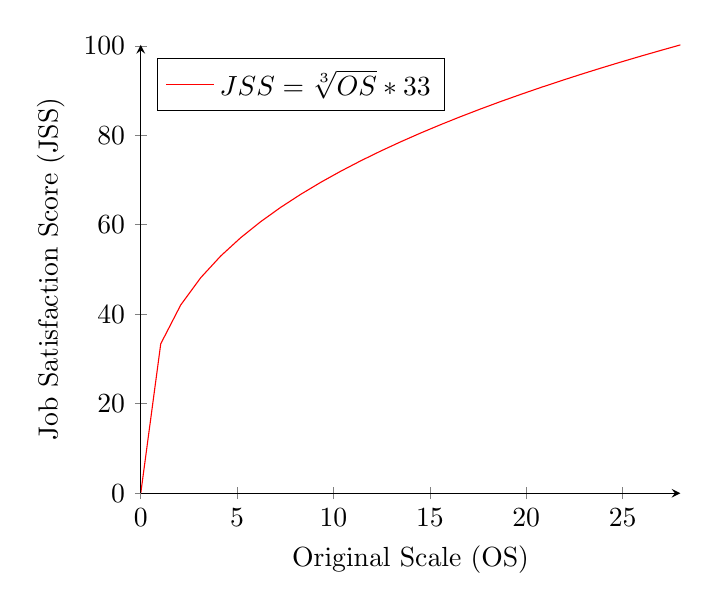
\begin{tikzpicture}
\begin{axis}[
    axis lines = left,
    xlabel = Original Scale (OS),
    ylabel = Job Satisfaction Score (JSS),
    grid style = dashed,
    legend pos=north west
]

\addplot [
    domain=0:28, 
    samples=28, 
    color=red,
]
{x^(1/3)* 33};
\addlegendentry{$JSS=\sqrt[3]{OS}*33$}
\end{axis}
\end{tikzpicture}

\subsubsection{Company Image}
The company image is a very important KPI to measure the company reputation. The company image is the sum of many small activities which leaves a footprint that can be recognized with the company. Single activities can improve or destroy the company image from the point of view of individuals. The goal of a high valued company image is of course monetary benefit. Therefore, activities which tend to increase the company image are not for free and it is always a difficult assessment whether to invest in a certain activity or not. In the game we concentrated on factors which can be realistically and interestingly be influenced by the player.

\begin{longtable}[]{l|c|c}
     \textbf{Action} & \textbf{Points} & \textbf{Monetary impact} \\
     \hline \hline
     \underline{\textbf{Social Engagement}} & & \\ [1ex]
     \multicolumn{1}{c|}{\textbf{CSR Donations (in \% of profit)}} & & Depending on profit \\
     No donations & 0 &  \\
     0 \% - 1 \% & 1 &  \\
     1 \% - 2 \% & 2 &   \\
     2 \% - 5 \% & 3 &   \\
     More than 5 \% & 4 &   \\ [1ex]
     \multicolumn{1}{c|}{\textbf{Support Refugee Projects}} & & \\
     Never & 0 &  \\
     1 project per year & 1 & -1000 \$ per year  \\
     2 projects per year & 2 & -2000 \$ per year   \\
     3 projects per year & 3 & -3000 \$ per year  \\
     4 projects per year & 4 & -4000 \$ per year  \\
     \hline \hline
     \underline{\textbf{Environmental Friendly Production}} & & \\ [1ex]
     \multicolumn{1}{c|}{\textbf{Supplier}} & & \\
     Eco-friendly & 2 & +10\% of cost \\
     Standard & 0 & 0\$  \\
     \multicolumn{1}{c|}{\textbf{Logistics Partner}} & & \\
     Eco-friendly & 2 & +10\% of cost \\
     Standard & 0 & 0\$  \\
     \hline \hline
     \underline{\textbf{Promotes a green image}} & & \\ [1ex]
     \multicolumn{1}{c|}{\textbf{Mandatory training for employees}} & & \\
     Never & 0 & 0 \\
     1 time per year & 1 & -1000\$ per employee  \\
     2 time per year & 2 & -2000\$ per employee  \\
     3 time per year & 3 & -3000\$ per employee  \\
     4 time per year & 4 & -4000\$ per employee  \\
     \multicolumn{1}{c|}{\textbf{Green marketing campaign}} & & \\
     Never & 0 & 0 \\
     1 time per year & 1 & -2500 \$  \\
     2 time per year & 2 & -5000 \$  \\
     3 time per year & 3 & -7500 \$  \\
     4 time per year & 4 & -10000 \$  \\
     \hline \hline
     \underline{\textbf{Promotes diversity}} & & \\ [1ex]
     \multicolumn{1}{c|}{\textbf{Mandatory diversity training}} & & \\
     Never & 0 & 0 \\
     1 time per year & 1 & -1000\$ per employee  \\
     2 time per year & 2 & -2000\$ per employee  \\
     3 time per year & 3 & -3000\$ per employee  \\
     4 time per year & 4 & -4000\$ per employee  \\
     \multicolumn{1}{c|}{\textbf{Diversity campaign}} & & \\
     Never & 0 & 0 \\
     1 time per year & 1 & -3000 \$  \\
     2 time per year & 2 & -6000 \$  \\
     3 time per year & 3 & -9000 \$  \\
     4 time per year & 4 & -12000 \$  \\
     \hline 
\caption{Actions influencing the Company Image}
    \label{tab:benefitsCIS}
\end{longtable}

The total sum of the above possible choices is the total Company Image Score (CIS). The score can reach values from 0 to 28 as it is the case for the Employee Satisfaction Score. In order to build also here a more realistic representation we figured out that the marginal benefit of an increase of the company image increases with the collected amount of points. Therefore, we manipulated also this formula and came up with the following function.

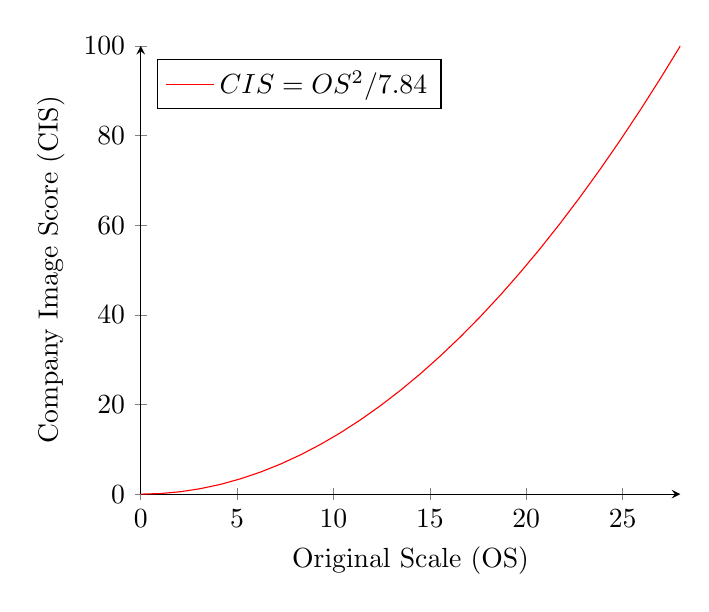
\begin{tikzpicture}
\begin{axis}[
    axis lines = left,
    xlabel = Original Scale (OS),
    ylabel = Company Image Score (CIS),
    grid style = dashed,
    legend pos=north west
]

\addplot [
    domain=0:28, 
    samples=28, 
    color=red,
]
{x^2/7.84};
\addlegendentry{$CIS=OS^2/7.84$}
\end{axis}
\end{tikzpicture}

The original scale of 0 to 28 is squared and divided by the factor of 7.84 in order to map the original scale on a scale of 0 to 100. In this case the rational behind the mapping is the fact that little activities do not have such  a big influence on the overall image of a company. When a company starts to combine all its activities it can generate huge impact and publicity which leads to a strong increase of the Company Image Score.

\subsubsection{Quality of Work}
The quality of work is a measure for the output quality of every process step in the corporation where an employee is involved. We are aware, that the quality of process outputs is influenced by more than the chosen factors here. However, for the sake of the realization of the game, we concentrated on the factors which can be chosen by a player simulating the role of a CEO or Chief Human Resources Officer (CHRO). Besides the influencing factors, which are defined and explained below, the skill level is the most important factor for the quality of an employee. The underlying assumption is that higher skilled employees have more experience and perform similar activities better than employees with a lower skilllevel in a comparable position.

The skilllevel becomes a strategic mechanism as it influences the quality of work significantly. In fact, a better quality of work leads to higher output of the production, can decrease product failure and improve the quality of the products, allows new products to be developed, and for example in case of sales employees generate more sales. 

The skilllevel alone is not enough to describe the influence on the Quality of work. The happiness and satisfaction with the job is also a measure that influences the quality of the delivered work by the employees.
Thus, the total quality of work is measured by an equal weighted average of the skilllevel and the job satisfaction. The skilllevel of employees can be influenced by trainings which is described in the section below.

\subsubsection{Training}
Emplyees can be categorized into 5 groups:
\begin{itemize}
    \item Worker (20)
    \item Student (30)
    \item Graduate (40)
    \item Specialist (60)
    \item Expert (80)
\end{itemize}
The initial skill level for these employees is set to (20, 30, 40, 60, 80) according to the order of the list above. In order to improve the skilllevel and by this the quality of work of the employees, training can be added to the learning journey of employees. 

Training can be assigned to a certain number of employees. The cost per training and also the increase of the skill level of the single employees depends on the kind of training. The courses are only relevant for employees of specific departments.

The following list summarizes the possible training which are offered and can be assigned to specific departments.
\begin{itemize}
\item The future of manufacturing- Production
\item Hot topics in manufacturing - Production
\item Lean production methods - Production, Logistics
\item Psychology of work - Sales, Marketing
\item Best practice in employer branding - Marketing, Sales
\item AIDA principle - Marketing, Sales
\item Environmental friendly processes - Production, Logistics
\item Sustainability in transport - Logistics
\item Persuasion techniques - Sales
\item Personality matters - Marketing, Sales
\end{itemize}

\subsubsection{Employer Branding}
The employer branding score is the score which is reported to the external world in order to measure the value of the company as an employer in total. This score is comparable to the total score for companies which is presented on websites like kununu or glassdoor. The employer branding is a combined score out of the Job Satisfaction and the Company Image. As the Company Image implicitly incluences the Job Satisfaction rating it is weighted with 0.4 in the calculation of the employer branding score. The general formula is
\begin{center}
$Employer Branding = 0.4 * CIS + 0.6 * JSS$ \\
with \\
CIS = Company Image Score   \\
JSS = Job Satiscation Score
\end{center}

In order to make the employer branding rating more realistic, we need to think about extreme cases where either the employee satisfaction or the company image is rated very low. The usage of a simple weighted average would have the effect that values of $JSS = 100$ and $CIS = 0$ lead to an overall score of 60.
Therefore we need to include an indicator function which incorporates a punishment for smaller values.
This can be done by incorporating a multiplier which is based on an IF statement. See the \textit{Excel} implementation below:
\begin{center}
    $=ROUND(((0.4*CIS+0.6*JSS)*IF(CIS<30,0.5,IF(CIS<60,0.8,IF(CIS>60,1))))/10,0)$
\end{center}

The following pseudo code explains the statement above.

\begin{itemize}
    \item score = 0.4*CIS + 0.6*JSS
    \item IF CIS $\leq$ 30 THEN Employer Branding = Employer Branding * 0.5
    \item ELSEIF CIS $\leq$ 60 THEN Employer Branding = Employer Branding * 0.8
    \item ELSEIF CIS $\geq$ 60 THEN Employer Branding = Employer Branding * 1
\end{itemize}

By this we ensure a sufficient punishment of the overall Employer Branding score. To achieve this we need to create a matrix and a 3D graph to visualize the possible implications on the employer branding. The following graphic shows the implications of the two input parameters on the Employer Branding.

\begin{figure}
	\centering
	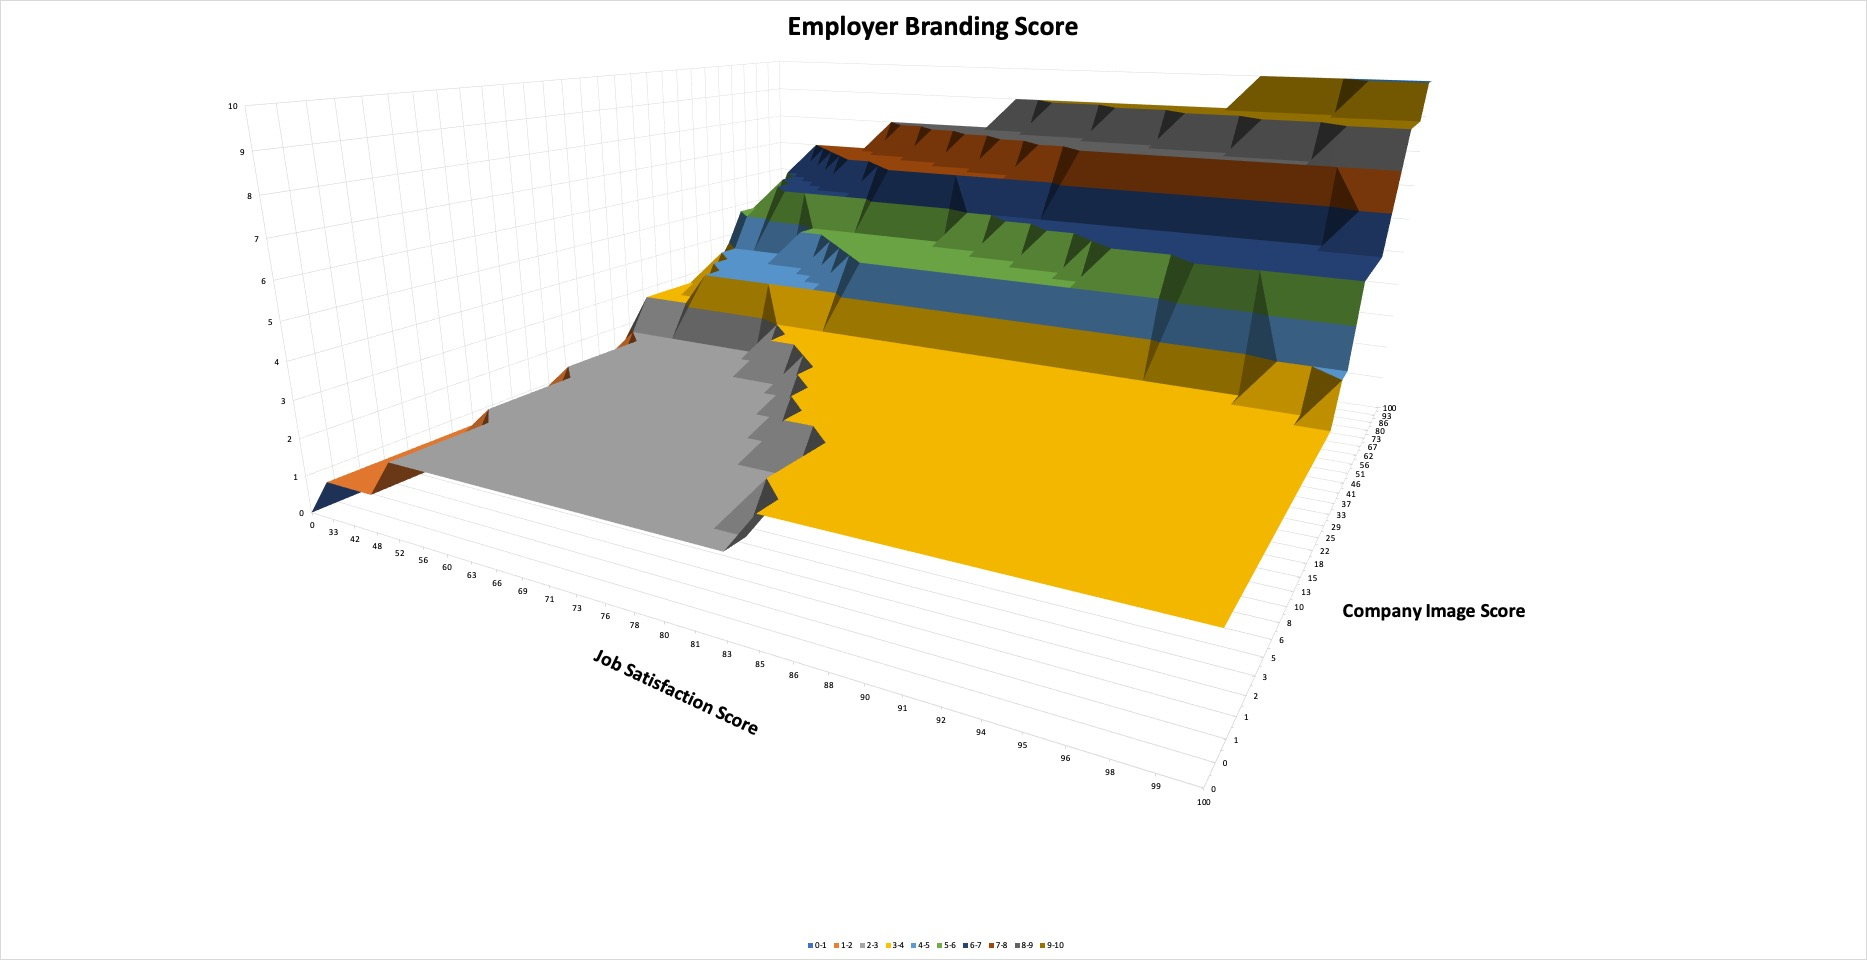
\includegraphics[width=12.5cm]{images/EBS.jpg}
	\caption{Employer Branding Score Caculation}
	\label{img:EBS}
\end{figure}

\subsection{Summary}

The single KPIs are calculated as follows: 
\begin{itemize}
\item Quality of Work = $JSS * 0.5 + Skilllevel * 0.5$
\item Skill Level = Initial Skill Level (based on employee category + influence training
\item Job Satisfaction Score (JSS) = Calculation based on JSS section above
\item Company Image Score (CIS) = Calculation based on CIS section above
\item Employer Branding = $JSS*0.6 + CIS*0.4$ and applying the punishment function. 
\end{itemize}